\documentclass[10pt]{beamer}

\usepackage{../macros}
\title{Ensembles et dictionnaires}

\hypersetup{
  pdftitle =  {Ensembles et dictionnaires}
}

\begin{document}

\maketitle


%%%%%%%%%%%%%%%%%%%%%%%%%%%%%%%%%%%%%%%%%%%%%%%%%%%%%%%
\begin{frame}[fragile]
  \frametitle{Où en sommes-nous des types de données ?}
  \begin{block}{Types simples}
  
  \begin{columns}[t]
\begin{column}{0.25\textwidth}
  \begin{lstlisting}
> class(42)
[1] "numeric"
  \end{lstlisting}
\end{column}
\begin{column}{0.25\textwidth}
  \begin{lstlisting}
> class(
as.integer(42))
[1] "integer"
  \end{lstlisting}
\end{column}


\begin{column}{0.25\textwidth}
  \begin{lstlisting}
> class(TRUE)
[1] "logical"
  \end{lstlisting}
\end{column}
\begin{column}{0.25\textwidth}
  \begin{lstlisting}
> class("42")
[1] "character"
  \end{lstlisting}
\end{column}
\end{columns}
\end{block}


\begin{block}{Types composés : séquence d'objets numérotés (\texttt{vector} et \texttt{list})}
  
\begin{columns}[t]
\begin{column}{0.48\textwidth}
  \begin{lstlisting}
> class(c(1,2,3))
[1] "numeric"    
  \end{lstlisting}
\end{column}
\begin{column}{0.48\textwidth}
  \begin{lstlisting}
> class(list('a',2,3))
[1] "list"    
  \end{lstlisting}
\end{column}
\end{columns}
\end{block}

\begin{alertblock}{Types composés : ensembles et dictionnaires.}
  \begin{itemize}
  \item Disponible dans de nombreux langages, mais pas en R.
  \item<alert@1> Nous allons les émuler grâce à des vecteurs et des listes nommés.
  \end{itemize}
\end{alertblock}
\end{frame}




%%%%%%%%%%%%%%%%%%%%%%%%%%%%%%%%%%%%%%%%%%%%%%%%%%%%%%%
\begin{frame}
  \frametitle{Les ensembles}
  \begin{figure}[t]
    \centering
    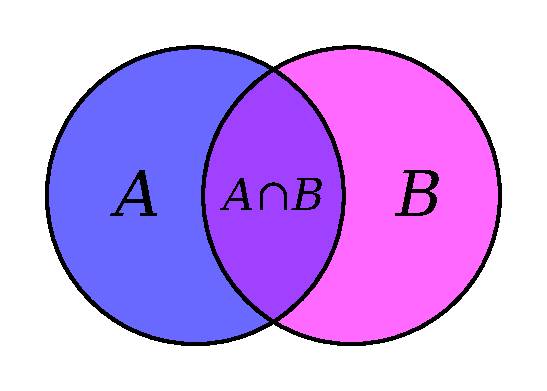
\includegraphics[width=0.6\textwidth]{Venn_A_intersect_B}
    \caption{Diagramme de Venn. \newline Origine : Georg Cantor (1845-1918), mathématicien allemand. }
  \end{figure}
\end{frame}

%%%%%%%%%%%%%%%%%%%%%%%%%%%%%%%%%%%%%%%%%%%%%%%%%%%%%%%
\begin{frame}[fragile]
  \frametitle{Qu'est-ce qu'un ensemble ?}

  \begin{alertblock}{Ensemble en R}
    Un ensemble en R est une séquence sans répétition et sans ordre (conceptuellement). 
    \begin{itemize}
    \item En théorie, les éléments sont de types quelconques.
    \item En pratique, on représente un ensemble (type simple) par un vecteur.
    \end{itemize}
\end{alertblock}



  \begin{exampleblock}{L'arithmétique des vecteurs ne suffit pas.}
    \begin{lstlisting}[style=block]
> 1:5 == 5:1 ## Vrai du point de vue ensembliste.
[1] FALSE FALSE  TRUE FALSE FALSE      
    \end{lstlisting}
  \end{exampleblock}


  \begin{block}{Égalité de deux ensembles}
    \begin{lstlisting}[style=block]
> setequal(1:5, 5:1)
[1] TRUE      
    \end{lstlisting}
  \end{block}
\end{frame}

%%%%%%%%%%%%%%%%%%%%%%%%%%%%%%%%%%%%%%%%%%%%%%%%%%%%%%%
\begin{frame}[fragile]
  \frametitle{Appartenance et cardinal d'un ensemble}

  \begin{block}{Appartenance d'un élément à un ensemble}
    \begin{lstlisting}[style=block]
> is.element(1, 1:5)
[1] TRUE
> is.element(0, 1:5)
[1] FALSE
\end{lstlisting}
  \end{block}

  \begin{exampleblock}{Cardinal d'un ensemble}
    Pas de fonction prédéfinie.
    \begin{lstlisting}[style=block]
> Cardinal <- function(x) length(unique(x))
> Cardinal(c(1:5, 1:5))
[1] 5
\end{lstlisting}
\end{exampleblock}

\end{frame}


%%%%%%%%%%%%%%%%%%%%%%%%%%%%%%%%%%%%%%%%%%%%%%%%%%%%%%%
\begin{frame}[fragile]
  \frametitle{Opérations sur les ensembles}
  \begin{block}{Union $A \cup B = \{x\ |\ x \in A\ \mathrm{ou}\ x \in B\}$}
    \begin{lstlisting}[aboveskip = \bigskipamount]
> union(1:5, 4:6)
[1] 1 2 3 4 5 6      
    \end{lstlisting}
  \end{block}

    \begin{block}{Intersection $A \cap B = \{x\ |\ x \in A\ \mathrm{et}\ x \in B\}$}
    \begin{lstlisting}[aboveskip = \bigskipamount]
> intersect(1:5, 4:6)
[1] 4 5
    \end{lstlisting}
  \end{block}

  \begin{block}{Différence asymétrique $A - B = \{x\ |\ x \in A\ \mathrm{et}\ x \notin B\}$}
    \begin{lstlisting}[aboveskip = \bigskipamount]
> setdiff(1:5, 4:6)
[1] 1 2 3
    \end{lstlisting}
  \end{block}

  \begin{exampleblock}{Inclusion $A \subseteq B \Leftrightarrow \left((\forall x \in A) \Rightarrow (x \in B)\right)$}
    \begin{lstlisting}[aboveskip = \bigskipamount]
> Inclusion <- function(x, y) setequal(x, intersect(x, y))
> Inclusions(5:6, 4:6)
[1] TRUE
    \end{lstlisting}
  \end{exampleblock}
  

\end{frame}


%%%%%%%%%%%%%%%%%%%%%%%%%%%%%%%%%%%%%%%%%%%%%%%%%%%%%%%
\begin{frame}
  \frametitle{Qu'est-ce qu'un dictionnaire ?}

  \begin{alertblock}{Dictionnaire en R}
    En théorie, un dictionnaire est une collection non numérotée de couples clé/valeur où la clé est un objet non mutable et la valeur est n'importe quelle valeur.
    \begin{itemize}
    \item Toutes les clés doivent être distinctes !
    \item R ne propose pas de classe pour les dictionnaires.
    \end{itemize}
    En pratique, nous allons \alert{émuler un dictionnaire} dont les clés sont des chaînes de caractères avec un \alert{vecteur nommé} ou une \alert{liste nommée}.  
  \end{alertblock}

  \begin{block}{Vecteurs et listes nommées}
    \begin{itemize}
    \item Écrire un code plus lisible.
    \item Utiliser les fonctions avancées de R (par ex. graphiques).
    \end{itemize}

  \end{block}
\end{frame}


%%%%%%%%%%%%%%%%%%%%%%%%%%%%%%%%%%%%%%%%%%%%%%%%%%%%%%%
\begin{frame}[fragile]
  % \frametitle{De l'utilité des dictionnaire \dots}
  \frametitle{Construction d'un dictionnaire}

\begin{block}{Construction en extension}
  On fournit tous les couples dans un ordre quelconque.
    \begin{lstlisting}[style=block]
> stock <- c(poires=51, pommes=243)
> print(stock)
poires pommes
51 243      
\end{lstlisting}
  \end{block}

  \begin{block}{Construction en deux temps}
    on fournit toutes les valeurs, puis tous les noms, dans le même ordre.
    \begin{lstlisting}[style=block]
> stock <- c(51,243)
> names(stock) <- c("poires", "pommes")
\end{lstlisting}
Remarquez que nous affectons les noms aux résultats d'une fonction !
\end{block}
\end{frame}


%%%%%%%%%%%%%%%%%%%%%%%%%%%%%%%%%%%%%%%%%%%%%%%%%%%%%%%
\begin{frame}[fragile]
  % \frametitle{De l'utilité des dictionnaire \dots}
  \frametitle{Accès aux valeurs d'un dictionnaire}
  \begin{alertblock}{Accès par clé}
  \begin{itemize}
  \item \alert{On peut accéder à la valeur associée à une clé.} 
  \item La recherche est pratiquement instantanée ! De la clé vers la valeur ! 
  \item La recherche est unidirectionnelle : Français --> Anglais.
  \end{itemize}
    \begin{lstlisting}
> stock['pommes']
250
> getElement(stock,"poires")
[1] 51    
\end{lstlisting}      
\end{alertblock}

\begin{columns}[t]
\begin{column}{0.4\textwidth}
\begin{block}{Accès par rang}
  \begin{lstlisting}[style=block]
> stock[1]
poires
51    
\end{lstlisting}    
\end{block}
\end{column}
\begin{column}{0.6\textwidth}
\begin{block}{Ne pas confondre rang et clé }
  \begin{lstlisting}[style=block]
> stock['1'] #ni clé, ni index
<NA>
NA
\end{lstlisting}    
\end{block}
\end{column}
\end{columns}

\end{frame}

%%%%%%%%%%%%%%%%%%%%%%%%%%%%%%%%%%%%%%%%%%%%%%%%%%%%%%%
\begin{frame}[fragile]
  \frametitle{Modification d'un dictionnaire }

\begin{block}{Modifier la valeur associée à une clé}
  \begin{lstlisting}[style=block]
> stock["pommes"] <- 250 
\end{lstlisting}
\end{block}

\begin{block}{Ajouter un nouveau couple clé/valeur}
  \begin{lstlisting}[style=block]
> stock["fraises"] <- 50
> print(stock)
poires pommes fraises
51 250 50    
\end{lstlisting}
\end{block}

\begin{block}{Attention, un dictionnaire est un vecteur !}
\begin{lstlisting}[style=block]
> c(stock, stock) # Les clés ne sont plus uniques !
 poires  pommes fraises  poires  pommes fraises 
     51     250      50      51     250      50   
   \end{lstlisting}
 \end{block}

 \begin{block}{Vérifier la présence d'une clé}
    \begin{lstlisting}[style=block]
> is.element("fraises", names(stock))
[1] TRUE
\end{lstlisting}
\end{block}


\end{frame}

%%%%%%%%%%%%%%%%%%%%%%%%%%%%%%%%%%%%%%%%%%%%%%%%%%%%%%%
\begin{frame}[fragile]
  \frametitle{Itérer dans un dictionnaire}
  \begin{block}{Accéder aux valeurs et aux clés}
    \begin{lstlisting}[style=block]
> unname(stock) # vecteur des valeurs sans les clés
[1]  51 250  50
> names(stock) # vecteur des clés
[1] "poires" "pommes" "fraises"    
\end{lstlisting}    
\end{block}

\begin{block}{Par défaut, on itère sur les valeurs}
\begin{lstlisting}[style=block]
> for(i in stock) {print(i)}
[1] 51
[1] 250
[1] 50  
\end{lstlisting}
\end{block}

\begin{block}{Mais, on peut itérer sur les clés}
\begin{lstlisting}[style=block]
> for(i in names(stock)) {print(i)}
[1] "poires"
[1] "pommes"
[1] "fraises"  
\end{lstlisting}
\end{block}
\end{frame}

%%%%%%%%%%%%%%%%%%%%%%%%%%%%%%%%%%%%%%%%%%%%%%%%%%%%%%%
\begin{frame}[fragile]
  \frametitle{Suppression dans un dictionnaire}
  \begin{block}{Suppression par clé}
    On ne peut pas directement supprimer la valeur associée à une clé.
    \begin{lstlisting}[style=block]
> stock[-'pommes']
Error in -"pommes" : invalid argument to unary operator    
\end{lstlisting}

  \end{block}

\begin{alertblock}{Émuler la suppression par clé}
  On va devoir trouver le rang de la clé, puis la supprimer par rang.
  Pour cela, on définir une fonction \texttt{remove(key)} qui renvoie le dictionnaire après suppression du couple key:val du dictionnaire.
  \begin{lstlisting}
Remove <- function(dict, key) {
 dict[ names(dict) != key]
}
\end{lstlisting}

\begin{lstlisting}
> Remove(stock, "pommes")
poires fraises
51 25  
\end{lstlisting}  
\end{alertblock}
\end{frame}


%%%%%%%%%%%%%%%%%%%%%%%%%%%%%%%%%%%%%%%%%%%%%%%%%%%%%%%
\begin{frame}[fragile]
  \frametitle{De l'utilité des dictionnaire \dots}
  On considère maintenant différentes variétés de chaque fruit.\\
  On ne peut plus utiliser un vecteur. On doit utiliser une liste.
  \begin{lstlisting}
> stock <- list(
  pommes = c(grany=25, golden=50, fujy=0),
  poires = c(comice=10, williams=100),
  fraises = c(marat=0, gariguette=100)
  )
\end{lstlisting}

\begin{block}{Accès par clé}
  \begin{lstlisting}[style=block]
> stock$fraises # accès par clé
     marat gariguette 
         0        100 
> stock[["fraises"]] # accès par clé
     marat gariguette 
         0        100 
> stock["fraises"] # extraction d'une tranche !
$fraises
     marat gariguette 
         0        100 
  \end{lstlisting}         
\end{block}
\end{frame}


%%%%%%%%%%%%%%%%%%%%%%%%%%%%%%%%%%%%%%%%%%%%%%%%%%%%%%%
\begin{frame}[fragile]
  \frametitle{Pour regarnir ses étals}
  Trouver les variétés dont le nombre de fruit est en dessous d'un seuil fixé.
  \begin{lstlisting}[style=editor]
  CommanderVarietes <- function(stock, seuil) {
   commandes <- c()
   for(fruit in stock) {
     varietes <- names(subset(fruit, fruit < seuil))
     commandes <- c(commandes, varietes)
   }
   return(commandes)
}
\end{lstlisting}

\begin{lstlisting}
> CommanderVarietes(stock, 50)
[1] "grany"  "fujy"   "comice" "marat" 
> CommanderVarietes(stock, 10)
[1] "fujy"  "marat"  
\end{lstlisting}
\end{frame}


%%%%%%%%%%%%%%%%%%%%%%%%%%%%%%%%%%%%%%%%%%%%%%%%%%%%%%%
\questionSlide

%%%%%%%%%%%%%%%%%%%%%%%%%%%%%%%%%%%%%%%%%%%%%%%%%%%%%%%
 \appendix
 \backupSlides
%%%%%%%%%%%%%%%%%%%%%%%%%%%%%%%%%%%%%%%%%%%%%%%%%%%%%%%

%%%%%%%%%%%%%%%%%%%%%%%%%%%%%%%%%%%%%%%%%%%%%%%%%%%%%%%
% \begin{frame}[fragile]{Backup slides}
%   Sometimes, it is useful to add slides at the end of your presentation to
%   refer to during audience questions.

%   The best way to do this is to include the \verb|appendixnumberbeamer|
%   package in your preamble and call \verb|\appendix| before your backup slides.

%   will automatically turn off slide numbering and progress bars for
%   slides in the appendix.
% \end{frame}


%%%%%%%%%%%%%%%%%%%%%%%%%%%%%%%%%%%%%%%%%%%%%%%%%%%%%%%
% \begin{frame}[allowframebreaks]{References}

%   % \bibliography{../bib_parallelism,../bib_others}
%   % \bibliographystyle{abbrv}

% \end{frame}

\end{document}

%%% Local Variables:
%%% mode: latex
%%% TeX-master: t
%%% End:
